\chapter{Introduction}\label{chapter:introduction}

\section{Explosion of biomedical data}

In recent times, there has been a phenomenal rise in the amount of information available in the world. Since scientific articles remains the preferred way of publishing scientific research, there has also been a huge increase in the volume of scientific literature, particularly in the area of biomedical sciences. PubMed \cite{pubmed}, the database of biomedical articles, boasts of more than 24 million scientific articles and is growing rapidly. In 2014 alone, PubMed have added more than a million articles. Figure \ref{fig:PubMedTimeLine} shows the growth of PubMed database in recent years.

\section{Need for automatic extraction of information}

With huge amount of information available in the biomedical literature, it has become impossible for researchers to keep track of all the developments in the field. Given the textual nature of this scientific literature, text-mining techniques are helping researchers to extract relevant information from this gold mine without having to read each and every article. As a result, there has been a tremendous increase in research in the area of text-mining biomedical literature. These techniques are intended to help the researchers who cannot manually scavenge thousands of articles for information.

\begin{figure}
\centering
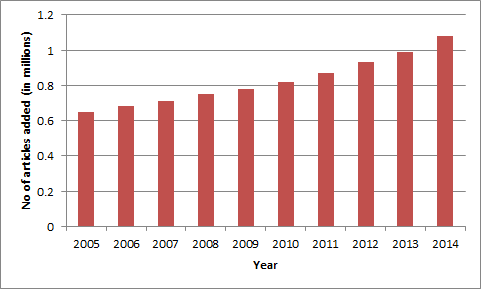
\includegraphics[scale=1]{figures/PubMedTimeLine.png}
\caption{Growth of PubMed in recent years}\label{fig:PubMedTimeLine}
\end{figure}

% TODO: 
\subsection*{Need for biomedical research community}
% 1. Write about why scientists both in biomedical and text-mining domain needs automatic information extractors. Need inputs on how this information

"Biomedical research" is an umbrella term used for research in various disciplines like biochemistry, immunology, microbiology, cytology, etc. To give an example, some of the problems studied in the area of biochemistry are protein-protein interaction, protein-ligand interaction, protein subcellular localization, etc. All of these different biochemical processes play a vital role in proper functioning of the body and any impairment in these processes can have far reaching effect on human health, usually blowing into a full-fledged disease. It is no wonder that many researchers across the globe are working simultaneously on some of these problems and therefore, it becomes essential for such researchers to keep track of the recent advances and start building from there. 

Conventionally, the best method to keep abreast of recent scientific advances is by reading the scientific literature. This remains the best way in some areas of science where the scientific throughput is less and harder to achieve. However in some fields like biomedical sciences, due to the huge volume of scientific literature, it has become very difficult for a researcher to stay updated about recent work being done in his area of interest. As pointed out by Cohen et.al. in \cite{cohen2005survey}, knowledge discovery requires extracting information from research articles. However, there is not a single individual in a position to go through the extraordinarily large volume of information manually.

Therefore, text-mining methods have a large role to play in assisting researchers to extract relevant information from the information trove. As the text mining methods cannot be 100\% accurate, the information is always extracted with certain degree of confidence.

\section{Subcellular localization of Proteins}

% Explain about why do we need to know about subcellular localization of proteins
The subcellular localization of proteins is one of the most studied biochemical processes. Proteins play a vital role in the functioning of cell machinery and are therefore called the "building blocks of life". The creation of proteins consists of two main phases, viz. transcription and translation. The proteins are created in the cytoplasm by flow of genetic information from DNA (Deoxyribonucleic acid) to RNA (Ribonucleic acid) and from RNA to proteins. The genetic information present in the DNA is converted to RNA by a process known as transcription. Transcription takes place in the nucleus of the cell. The RNA strand so created, travels from nucleus to cytoplasm through the nuclear pores. In the cytoplasm, RNA strand is used to create a protein with the help of cellular machinery called as ribosomes. The process of converting RNA to a chain of amino acids called proteins is called translation. 

Although the proteins are created in the cytoplasm, they do not necessarily perform their biological functions in the cytoplasm. A protein can perform its function anywhere in the cell (cytoplasm or cellular organelle) or outside the  cell. The biological function of proteins largely depend on their location and therefore, knowledge of the subcellular location of a protein is key to understanding its biological function. The subcellular location is a generic term used to indicate the location, even if the protein exits the cell and performs its  function outside the cell.

\subsection{Important role in drug research}
% 2. How automatic extraction of information will help in drug research

Proteins play a very important role in proper functioning of the cell machinery and hence, an abnormality in their functioning can result in adverse effects, even leading to a disease. The study of proteins and their subcellular location is an important stage in the development of a drug. Drug researchers study the subcellular location of proteins, which can help them identify suitable drugs, vaccines or diagnostic treatments \cite{liu2007exploiting}. 


\subsection{Current sources of information}
% Explain about 
%- Uniprot, Swissprot and Trembl. 
%- Also talk about the procedure followed by PubMed annotators and how locations are mentioned for each protein
%- Can also talk about sources where you can extract protein-location relation

Currently, important sources of information about subcellular location of proteins are knowledge bases like UniProtKB \cite{magrane2011uniprot}, manual curation from the literature, high-throughput microscopy-based screens and prediction from primary (protein) sequence.

\subsection{Need of automatic extraction}

Although knowledge bases like UniProtKB \cite{magrane2011uniprot} have considerable amount of information about proteins, including their subcellular location, it is not complete and can be supplemented \cite{goldberg2015linked}. UniProtKB consists of two sections, viz. Swiss-Prot and TrEMBL. TrEMBL contains automatically annotated information about a protein whereas Swiss-Prot contains the information which is manually reviewed by a curator. Every curator is in charge of certain proteins and he/she extracts the information manually by reading the literature. Obviously, this process is cumbersome and time-consuming. In addition, owing to the large amount of articles being published daily, it is impossible for these curators to update the information in the database constantly. This often results in some lag between the information present in knowledge bases and information in most recent literature.

Automatic text-mining methods can help the manual curators as well as the researchers to keep them updated about the information that is not present in the knowledge bases. The extraction of information about subcellular locations of proteins can also help experimental biologists to verify this information experimentally. The information might also be useful to predict the location of other proteins, which have considerable sequence similarity with the protein whose information is extracted by text-mining.

\subsection{Development of a new method}

In this thesis, I have developed a new method to extract the subcellular locations of proteins, automatically from the literature using text-mining techniques. This task involves extracting the semantic relationship between the entities, viz. protein and subcellular location, present in the text. Therefore, this process of extracting information is also called as relationship extraction. Throughout the rest of this document, the term "protein-subcellular location relation" is shortened  as "protein-location relation" for brevity.

Section \ref{sec:existingWork} describes previous work done in this area. Chapter \ref{chapter:corpus} describes the process of data set annotation and the insights obtained during manual annotation. Chapter \ref{chapter:theory} explains the theoretical background of the methods described in Chapter \ref{chapter:methods}. The results of the method and the conclusions derived are discussed in Chapter \ref{chapter:results} and Chapter \ref{chapter:conclusion} respectively.

\section{Related work}\label{sec:existingWork}

There has been little work done to solve the exact problem of protein-location relation extraction. However, there are some research groups that have done related work. This section presents an overview of the recent work done concerning this problem.

%Literature Survey
\subsection{Using syntactic trees for relation extraction - Liu et al.}

Liu et al. \cite{liu2007exploiting} proposed a method for extraction of protein-organism (PO) relations and protein-location (PL) relations from text using syntactic parse trees. The protein-organism (PO) and protein-location (PL) relations are then merged to create a ternary protein-organism-location (POL) relation. This is the single work that focused on the exact same problem that I tried to solve, i.e., protein-location relation extraction.

The corpus used in this method consisted of MEDLINE titles and abstracts annotated by domain expert biologists and parsed by the Charniak-Johnson parser \cite{charniak2006multilevel}. The work focused only on extracting same sentence relations. Two models were developed for the extraction of relations, viz. Semantic Role Labeling based relation extraction (SRL) model and Tree kernel based relation extraction (TRK) model. 

The SRL model used manually-extracted features from syntactic parse trees. These features were extracted along the path from protein to location/organism in the syntactic parse tree. The model was then trained by a Binary SVM using default linear kernel from Joachim’s SVM light \cite{joachims1999making}. Finally, the binary relations, viz. PO (protein-organism) and PL (protein-location) were fused together to form a ternary relation POL (protein-organism-location). The TRK model used entire parse tree as input for tree kernel. The model was trained using default tree kernel from Moschetti’s SVM-light-TK-1.2 \cite{moschitti2004study}. 

\begin{figure}
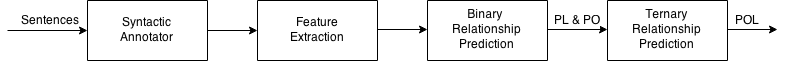
\includegraphics[scale=0.5]{figures/Liu_Flow.png}
\caption{Flow of information in method by Liu et al.}\label{fig:LiuFlow}
\end{figure}

Figure \ref{fig:LiuFlow} shows the overall flow of information. Best results were obtained when the prediction of both the models, viz. SRL and TRK were fused together. Table \ref{tab:LiuRes} shows the results for combination of both models. Since the method focused exclusively on same-sentence relations, it is not clear whether the results were calculated considering inter-sentence relations or not.

\begin{table}
\centering
\begin{tabular}{|l|l|l|l|l|}
\hline
\textbf{Relation} & \textbf{Precision} & \textbf{Recall} & \textbf{Fscore} & \textbf{Accuracy} \\ \hline
\textbf{PL} & 74.9 & 79.4 & 77.1 & 72.8 \\
\textbf{PO} & 73.9 & 78.1 & 75.9 & 72.6 \\
\textbf{POL} & 75.3 & 74.5 & 74.9 &  71.8\\ \hline
\end{tabular}
\caption{Results of combined prediction from models SRL \& TRK}\label{tab:LiuRes}
\end{table}

\subsection{BioNLP shared task and localization events}
% Explain what BioNLP event is and how localization is one of the 9 events that are meant to be extracted automatically

The BioNLP shared task events were organized in 2009 \cite{kim2009overview}, 2011 and 2013 to gauge the progress of the biomedical text-mining community on various information extraction tasks. These events were organized like a contest where research teams across academia and industry were invited to submit prediction results for a given task. 

The BioNLP event organizers provided an annotated corpus to the the text-mining community and invited solutions for the tasks. One of the tasks was shared task,  which involved extraction of the biological events present in the text. The data used for the shared task in BioNLP 2009 was a subset of the GENIA event corpus \cite{kim2008corpus}. The corpus was annotated for several biological events, one of which was \textit{Localization} and therefore, the methods employed in these BioNLP events can be an important source of study for the purpose of protein-location relation extraction.

\subsubsection{Event extraction}

\begin{figure}
\centering
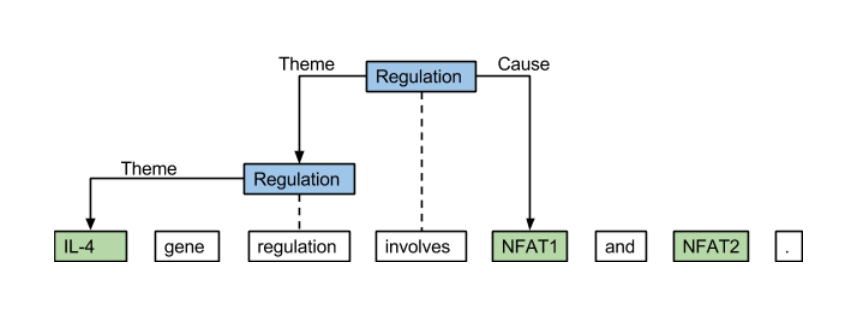
\includegraphics[scale=0.4]{figures/EventExample.png}
\caption{Example of an event in Biomedical Text}\label{fig:eventExample}
\end{figure}

Figure \ref{fig:eventExample} shows an example event from biomedical text. The sentence "IL-4 gene regulation involves NFAT1 and NFAT2." is \textit{tokenized} (divided into single word units or \textit{tokens}) and every token is shown as a rectangle in the figure. The protein tokens are shown in green rectangles and the events are represented with blue rectangles.

The task of event extraction from biomedical text can be broken down into the following subtasks:

\begin{enumerate}

\item \textbf{Trigger extraction:} This step involves extracting \textit{triggers} from the text and classifying them into appropriate event category. \textit{Triggers} are tokens or set of tokens in the text that give a clue about the presence of a biological event. For example, in Fig. \ref{fig:eventExample}, tokens "regulation" and "involves" are event triggers for the event \textit{Regulation}.

\item \textbf{Argument extraction: } This step involves extracting the arguments for already extracted triggers. The argument can be a named entity such as a protein or it can be another event trigger. In this step, all event triggers or named entities in the vicinity of an event trigger are considered as potential arguments and the relationship between the original event trigger and the potential argument is classified into one of the possible relation categories, i.e., $\left\lbrace Theme, Cause, NIL \right\rbrace$ where $NIL$ implies no relationship.

For example, in Fig. \ref{fig:eventExample}, the \textit{Regulation} event with trigger word "regulation" has a single theme argument to the token "IL-4". The \textit{Regulation} event with trigger word "involves" has two arguments, a theme argument to another event \textit{Regulation} and a cause argument to the named entity "NFAT1".

\item \textbf{Event construction: }  The last subtask in the process of event extraction is to construct proper events from event triggers and their arguments. The construction of events is determined by rules, which are specific to an event. Some regulation events such as \textit{Regulation}, \textit{Positive\_regulation} and \textit{Negative\_Regulation} can have two arguments, a theme and a cause whereas events like \textit{Gene\_expression} and \textit{Transcription} strictly have only one theme argument, which must be a named entity.

Figure \ref{fig:eventExample} shows two \textit{Regulation} events.

\end{enumerate}

\subsubsection{Difference between \textit{Localization} event extraction and protein-location relation extraction}

Although the task of \textit{Localization} event extraction is quite similar to the task of protein-location relation extraction, there are subtle issues in the GENIA event corpus which disallow using the same corpus and the same methods for the task of protein-location relation extraction.

Following are some of those issues:

\begin{enumerate}

\item Not all the locations found in the GENIA event corpus are subcellular locations. Some of them are even specific cells or tissues in the body.

\item Some \textit{Localization} events are annotated without any mention of the subcellular location but only due to the fact that the text contains some clues for \textit{Localization} event.

\item The location mention contains extraneous words that are a part of the phrase but not absolutely essential for location mention.

\end{enumerate}

Due to all these problems, I decided not to use the GENIA event corpus for my task. I, along with my team, decided to develop a corpus specifically tailored for the task of protein-location relation extraction to develop the method using it.

\subsubsection{State of the art in BioNLP'09} \label{sec:JariBioNLP}
%Work of Björne et al

The method developed by Björne et al. \cite{bjorne2009extracting} registered the-state-of-the-art performance in BioNLP Shared Task Event 2009. The method focused only on the events present in the same-sentence. As per their claim, about 95\% of the events are fully contained in a single sentence and therefore, it is sufficient \& relatively simpler to extract only same sentence events.

The method heavily uses the dependency parses of the sentence. It represents a sentence as a graph where the text tokens in the sentence are the nodes of the graph and the dependencies among the tokens are the edges in the graph. The model is trained by a rich set of features extracted from the graph. For every stage of event extraction, somewhat different set of features are used. 

The sentences are tokenized and parsed before processing. The method works in three stages as follows: 

\begin{enumerate}
\item \textbf{Trigger recognition}: The SVM (Support Vector Machine) model trained for this step classifies the tokens in the sentence into one of the event categories or none.

\item \textbf{Argument/Edge detection}: Every potential edge from one event trigger to another event trigger and from an event trigger to a named entity is classified into theme, cause or negation. This step uses a different SVM model than what is used in the step of trigger recognition.

\item \textbf{Semantic post-processing}: This step reconstructs the events and converts them into the appropriate format ( e.g. BioNLP 2009 format). It also removes irrelevant edges. 
\end{enumerate}

The method used the BioNLP event corpus as the dataset and Joachim's SVM Light \cite{bjorne2009extracting} for multiclass classification. 

Following are the results of the method developed by Björne et al.:

\begin{table}[h]
\centering
\begin{tabular}{|l|l|l|l|l|}
\hline
\textbf{Event Class} & \textbf{\# Events} & \textbf{Recall} & \textbf{Precision} & \textbf{Fscore} \\ \hline
\textbf{Localization} & 174 & 49.43 & 81.90 & 61.65 \\
\textbf{Total} & 3182 & 46.73 & 58.48 & 51.95\\ \hline
\end{tabular}
\caption{Results of the Graph-based event processing}\label{tab:Jari}
\end{table}

There were a total of nine events but only \textit{Localization} event results are shown for reference in Table \ref{tab:Jari}.

\subsubsection{Using Markov Logic Networks for event extraction (Yashikawa et al.)}

Extending the results of Björne et al., Yashikawa et al. \cite{yoshikawa2011coreference} used coreference resolution to extract events that span over multiple sentences in addition to extracting events from the same sentence. 

Yashikawa et al. uses the GENIA event corpus instead of the BioNLP'09 corpus since the GENIA corpus provides proper cross-sentence coreferences. They show that the SVM multiclass method proposed by Björne et al. gives better results if coreference annotation is used. In addition, they also developed a new model based on joint Markov Logic Network (MLN) which improved the results significantly.

To extract inter-sentence relations, the property of transitivity is used in the following way:

%TODO: Write in formulation
$$
\text{relation} \left( i,j,r \right) \land \text{corefer} \left(j,k \right) \implies \text{relation} \left( i,k,r \right)
$$

To put in plain words, if there is a relation $r$ between an event trigger $i$ \& a token $j$ in the sentence and if the token $j$ has an antecedent $k$ (which can be a named entity or event trigger) that can be resolved through anaphora or coreference resolution, then there is a relation $r$ between an event trigger $i$ and that antecedent $k$.

The GENIA event corpus consists of thirty-five event classes. For the task of event extraction from the GENIA corpus, MLN model achieves a F1 score of 53.8 with naive coreference resolver and 56.7 with gold coreference annotation. The results of MLN model are better than the results of model developed by Björne et al. The model developed by Björne et al. could achieve a F1 score of 51.95 for the task of event extraction from BioNLP corpus, which consisted of only nine event classes.

\subsection{COMPARTMENTS}

%Write about compartments 
%- Imai K etal. compartment reference 19
%- BacelLo compartment reference 20

Binder et al. \cite{binder2014compartments} designed the COMPARTMENTS resource,  which integrates protein-location relations from different sources such as databases and prediction tools. Although this method doesn't rely solely on text-mining, it is worth mentioning since it is the most recent work in this area. To create a uniform representation of the information collected from different sources, the proteins and the subcellular localizations are mapped to common protein identifiers and GO Ontology terms respectively. A confidence score is assigned to the localization evidence to enable comparison of different types and sources of evidence. The unified location evidence for a protein is then visualized on a schematic cell to  provide a simple overview.

There are different channels or sources from which the information is collected. The first channel is a \textit{knowledge} channel which contributes information based on the annotations from databases like UniProtKB, MGI, SGD, FlyBase, and WormBase. The second channel of information called \textit{experiments} is based on HPA (Human Protein Atlas), which is an ongoing effort to experimentally validate  the tissue expression and subcellular localization for entire set of human proteins. The third channel which is of particular interest for me is \textit{automatic text mining} and the fourth channel of information is \textit{predictions} which depends on prediction of subcellular location from protein sequence.

The \textit{automatic text mining} channel contributes the information extracted by a text-mining method. The text-mining method, which extracts the information from MEDLINE abstracts works on the supposition that, the more the protein and the cellular compartment is co-mentioned, the more likely the protein is localized to that compartment. This leads to the calculation of a score that determines the confidence of a protein being localized to a cellular compartment.

\section{Need for a dedicated method}
%
%- Explain about how localization event extraction tasks differ from our task
%- Explain about how coreference resolution takes a lot of time and isn't really accurate
%- Explain how many of the PL relations can exist outside same sentence

As mentioned previously, the GENIA event corpus or the BIONLP shared task corpus cannot be directly used for extracting protein-location relations. Therefore, there is a need to have a dedicated corpus designed for the purpose of training the text-mining method. In addition, using the nuances of new corpus, the method can produce better results.

%Although, the model developed by Yashikawa et al. extracts relations spanning over multiple sentences, extracting coreference information from the text at run-time is slow. 

Therefore, I decided to develop a dedicated text-mining method to extract protein location relations present in the corpus. I focused not only on  same-sentence relations but also on different-sentence relations in which the participating entities are in different sentences. As discussed in section \ref{sec:corpusStats}, we found out that around 40\% of total relations cross sentence boundaries and therefore, developing a method that would consider different sentence relations would help us to extract more relations from the data.




















%The relation between PROTEIN and LOCALIZATION tells about the location where the protein may lie. The location can be a subcellular location as well as it can be an extracellular location. The location of PROTEIN is closely associated with its biological function and an ability to predict its location will be helpful to identify suitable drug, vaccine and diagnostic treatment ~\parencite{liu2007exploiting}. \citep{liu2007exploiting}. The prediction of protein location can also be extrapolated to some proteins for which localization is not known but it holds structural similarity with proteins for which localization are known. Therefore, in context of natural language processing, the problem of relation extraction between a protein and localization can be put simply as: recognizing whether a "protein" lies in the "location" if the words "protein" and "location" are found in the biomedical text that is being processed.
%
%The key problem while developing text mining tools on biomedical texts is the availability of annotated corpus. However, the advent of GENIA corpus\citep{kim2003genia} have facilitated the development of text mining methods. With the availability of GENIA event corpus \citep{kim2008corpus} and introduction of BioNLP'09 shared task data\citep{kim2009overview}, research in the area of event extraction has intensified. One of the events addressed in the areas of event extraction is localization. However, localization event extraction techniques concentrate mainly on events that change the location of biological entities such as protein. They do not focus so much on the existing state of localization of protein. Therefore, the problem of relation extraction that we are trying to address is not similar to event extraction proposed in BioNLP'09 Shared Task.
%
%There has been some research in the areas of relation extraction with respect to protein localization \citep{liu2007exploiting}. However, they do not take into account cross sentence relations. There have also been some research as a sub problem addressed in event extraction techniques \citep{bjorne2009extracting} \citep{yoshikawa2011coreference}. However, they do not focus solely on relation extraction and have developed their method to be able to address event extraction as a whole. Therefore, there is need to develop a text mining approach which addresses the problem of relation extraction for protein localization while considering inter-sentence as well as intra-sentence relations.


%\section{Section}
%Citation test~\parencite{latex}.

%\subsection{Subsection}
%See~\autoref{fig:sample}.
%
%\begin{figure}[htsb]
%  \centering
%  
\includegraphics{logos/tum}
%  \caption[Example figure]{An example for a figure.}\label{fig:sample}
%\end{figure}
%
%\section{Section}
%
%See~\autoref{tab:sample}, \autoref{fig:sample-drawing}, \autoref{fig:sample-plot}, \autoref{fig:sample-listing}.
%
%\begin{table}[htsb]
%  \caption[Example table]{An example for a simple table.}\label{tab:sample}
%  \centering
%  \begin{tabular}{l l l l}
%    \toprule
%      A & B & C & D \\
%    \midrule
%      1 & 2 & 1 & 2 \\
%      2 & 3 & 2 & 3 \\
%    \bottomrule
%  \end{tabular}
%\end{table}
%
%\begin{figure}[htsb]
%  \centering
%  % This should probably go into a file in figures/
%  \begin{tikzpicture}[node distance=3cm]
%    \node (R0) {$R_1$};
%    \node (R1) [right of=R0] {$R_2$};
%    \node (R2) [below of=R1] {$R_4$};
%    \node (R3) [below of=R0] {$R_3$};
%    \node (R4) [right of=R1] {$R_5$};
%
%    \path[every node]
%      (R0) edge (R1)
%      (R0) edge (R3)
%      (R3) edge (R2)
%      (R2) edge (R1)
%      (R1) edge (R4);
%  \end{tikzpicture}
%  \caption[Example drawing]{An example for a simple drawing.}\label{fig:sample-drawing}
%\end{figure}
%
%\begin{figure}[htsb]
%  \centering
%
%  \pgfplotstableset{col sep=&, row sep=\\}
%  % This should probably go into a file in data/
%  \pgfplotstableread{
%    a & b    \\
%    1 & 1000 \\
%    2 & 1500 \\
%    3 & 1600 \\
%  }\exampleA
%  \pgfplotstableread{
%    a & b    \\
%    1 & 1200 \\
%    2 & 800 \\
%    3 & 1400 \\
%  }\exampleB
%  % This should probably go into a file in figures/
%  \begin{tikzpicture}
%    \begin{axis}[
%        ymin=0,
%        legend style={legend pos=south east},
%        grid,
%        thick,
%        ylabel=Y,
%        xlabel=X
%      ]
%      \addplot table[x=a, y=b]{\exampleA};
%      \addlegendentry{Example A};
%      \addplot table[x=a, y=b]{\exampleB};
%      \addlegendentry{Example B};
%    \end{axis}
%  \end{tikzpicture}
%  \caption[Example plot]{An example for a simple plot.}\label{fig:sample-plot}
%\end{figure}
%
%\begin{figure}[htsb]
%  \centering
%  \begin{tabular}{c}
%  \begin{lstlisting}[language=SQL]
%    SELECT * FROM tbl WHERE tbl.str = "str"
%  \end{lstlisting}
%  \end{tabular}
%  \caption[Example listing]{An example for a source code listing.}\label{fig:sample-listing}
%\end{figure}
